% Template for specification of a thesis (HTL Weiz edition)
% by Christian Schorna, 2022
\documentclass[12pt, draft]{article}
\usepackage{specStyle}

\begin{document}

\input{titlePage.tex}

\section*{Projektteam}
\begin{tabularx}{\textwidth}{| >{\hspace{0pt}}p{0.15\textwidth} | >{\hspace{0pt}}p{0.21\textwidth} | >{\hspace{0pt}}p{0.15\textwidth} | X |}
    \hline
    \textbf{Name} & \textbf{Individuelle Themenstellung} & \textbf{Telefon} & \textbf{E-Mail} \\
    \hline

    Nachname Vorname &  & +43 xxxxxxxxxx & christian.Schorna@hotmail.com \\
    \hline
    Nachname Vorname &  & +43 xxxxxxxxxx & E-Mail \\
    \hline
\end{tabularx}

\section*{Betreuer/innen}
\begin{tabularx}{\textwidth}{| >{\hspace{0pt}}p{0.15\textwidth} | >{\hspace{0pt}}p{0.15\textwidth} | >{\hspace{0pt}}p{0.15\textwidth} | X |}
    \hline
    \textbf{Rolle} & \textbf{Name} & \textbf{Telefon} & \textbf{E-Mail} \\
    \hline
    Hauptverantwortlich & Nachname Vorname (KZ1) & +43 xxxxxxxxxx & christian.schorna@hotmail.com \\
    \hline
        & Nachname Vorname (KZ2) & +43 xxxxxxxxxx & E-Mail Adresse \\
    \hline
\end{tabularx}

\section*{Projektpartner}
\begin{center}
    \begin{tabularx}{\textwidth}{| >{\hspace{0pt}}p{0.2\textwidth} | >{\hspace{0pt}}p{0.15\textwidth} | >{\hspace{0pt}}p{0.15\textwidth} | X |}
        \hline
        \textbf{Firmenname} & \textbf{Name} & \textbf{Telefon} & \textbf{E-Mail} \\
        \hline
         & Nachname Vorname & +43 xxxxxxxxxx & E-Mail Adresse \\
        \hline
    \end{tabularx}
\end{center}

\section*{Versionskontrolle}
\begin{tabularx}{\textwidth}{| p{0.1\textwidth} | p{0.125\textwidth} | p{0.15\textwidth} | X |}
    \hline
    \textbf{Version} & \textbf{Datum} & \textbf{Autor(en)} & \textbf{Änderungsgrund / Bemerkungen} \\
    \hline
    0.1 & 01.01.2022 & KZ1, KZ2 & Ersterstellung als Diskussionsgrundlage \\
    \hline
    0.2 & 01.01.2022 & KZ1 & Erste Revision \\
    \hline
    1.0 & 01.01.2022 & KZ2 & Endversion \\
    \hline
    1.1 & 01.01.2022 & KZ1, KZ2 & Endversion als Diskussionsgrundlage \\
    \hline
\end{tabularx}
\clearpage

\fancyhead{} % clear header
\tableofcontents
\clearpage

\section{Allgemeines - Zweck und Ziel dieses Dokuments}
In diesem Dokument wird festgehalten, welche Arbeiten im Rahmen des Projekts zu erledigen sind.
Dazu werden konkrete Fälle explizit ein- oder ausgeschlossen.
Zur besseren Übersicht befindet sich im Anhang eine stichwortartige Aufzählung der zu erledigenden Arbeiten.
Die Anforderungen sind dabei in Muss- und Optionale Punkte unterteilt. \\
\textbf{Auf die Implementierung wird im Pflichtenheft nicht eingegangen.}

\section{Informationen für die Projektdatenbank}
\subsection{Ausgangslage}
Beschreibung der IST Situation, der Problemstellung bzw. den Anlass für das Projekt.
Die Beschreibung der Ausgangslage soll verständlich machen warum das Vorhaben relevant und notwendig ist (z.B. ist das Projekt innovativ, gibt es bereits ähnliche Projekte, kann auf bereits gesammelte Erfahrungen aufbaut werden, usw.).

\subsection{Partner und Betreuungspersonen}
Beschreibung der Partnerinstitutionen und deren Vertreter.

\subsection{Untersuchungsanliegen der individuellen Themenstellung}
Hier wird erörtert, was durch dieses Projekt z.B. beschrieben, gebaut, überprüft oder geklärt werden soll.
Es soll auch beschrieben werden, wie das Projekt durchgeführt wird und welche konkreten Aktivitäten geplant sind. \\
Individuell pro Themenstellung!!

\subsection{Zielsetzung}
Beschreibung der beabsichtigten Ziele des Projektes.
Die Zielsetzung gibt Auskunft darüber, was Sie mit dem Projekt erreichen möchten.
Die Norm definiert das Projektziel als „Gesamtheit von Einzelzielen, die durch das Projekt erreicht werden“.

\subsection{Geplantes Ergebnis der Prüfungskandidaten/des Prüfungskandidaten}
Bei der Definition der geplanten Ergebnisse ist es sinnvoll, sich auch über deren Überprüfbarkeit Gedanken zu machen, also Indikatoren zu überlegen, an Hand derer man die Erreichung des Zieles erkennen kann.
Es sollen konkrete, messbare Maßnahmen definiert werden. \\
Individuell pro Themenstellung!!

\subsection{Projektbezug}
Hier wird die Grundidee des Projekts beschrieben;
in welchem Umfeld Sie eingesetzt wird, wozu sie gut ist, etc.

\section{Zielkriterien}
\subsection{Hardwarespezifikation}
Hier wird beschrieben, wie die Hardware aufgebaut sein soll, beziehungsweise was das Gerät hardwaretechnisch können soll!
\begin{itemize}
    \item Ist ein PC oder ein Mikrocontroller in Verwendung?
    \item Ist es ein transportables Gerät oder fix verbaut?
    \item Gibt es besondere Schutzmaßnahmen oder Gehäuseanforderungen?
\end{itemize}

\subsubsection{Human Machine Interface (HMI)}
Eine Beschreibung was der Nutzer manuell am Gerät machen kann.
\begin{itemize}
    \item Welche Bedienelemente gibt es?
    \item Wie wird das Gerät betrieben?
\end{itemize}

\subsection{Softwarespezifikation}
Hier wird beschrieben, wie die Software aufgebaut sein soll, beziehungsweise was das Gerät softwaretechnisch können soll!
\begin{itemize}
    \item Programmiersprache
    \item Grober Softwareaufbau
    \item Sonstige Features
\end{itemize}

\subsubsection{Human Machine Interface (HMI)}
Eine Beschreibung der Möglichkeiten zur Beeinflussung des Betriebs des Gerätes.
\begin{itemize}
    \item Beschreibung Menüführung mit den Ebenen
    \item Unterschiedliche Betriebsmodi (Normal-, Automatik-, Einzelschritt-, Expertenbetrieb)
\end{itemize}

\subsection{Test und Industrialisierung}
Beschreibung, wie die Funktion des Gerätes oder der Anlage über den geforderten Arbeitsbereich sichergestellt werden kann. \\
Dazu ist ein Konzept notwendig, das den Test und die Vermessung der notwendigen Parameter definiert.
Wenn notwendig auch über eine zu definierende Anzahl an Geräten hinweg, um statistische Auswertungen machen zu können.

\subsection{Maschinensicherheit}
Hier soll ein Bezug zur Maschinensicherheitsrichtlinie beziehungsweise zu einer eventuell notwendigen CE-Zertifizierung hergestellt werden.

\section{Erweiterte Ziel- oder Wunschkriterien}
Beschreibung was über die Normalanforderung an das Projekt noch realisiert werden könnte.

\section{Geräteaufbau}
\subsection{Blockschaltbild der Hardware}
Hier wird beschrieben, wie die Hardware in Blöcken aufgebaut sein soll, beziehungsweise was in welchen Baugruppen bearbeitet oder ausgewertet wird! \\
Auch das Thema EMV kann hier behandelt werden.
\begin{figure}[h]
    \centering
    % 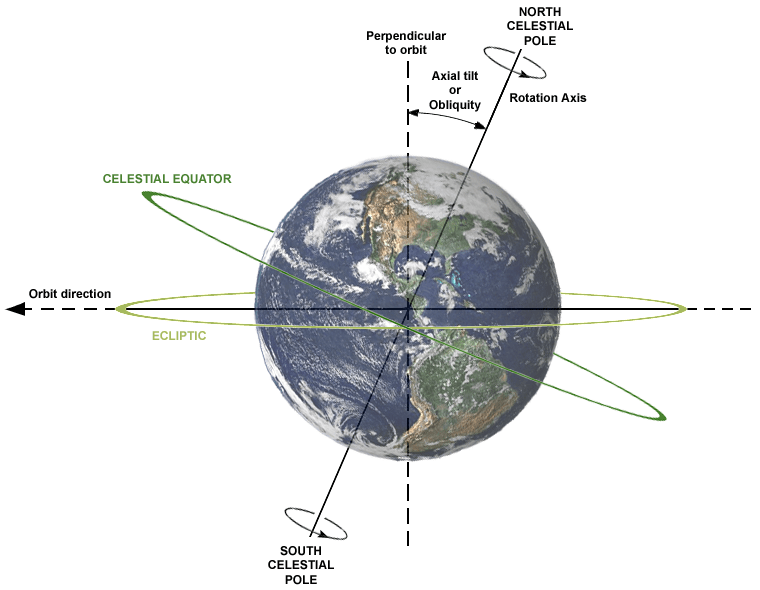
\includegraphics[width=100mm]{fig/earthOrbit}
    \caption{Blockschaltbild der Hardware}
\end{figure}
\begin{figure}[h]
    \centering
    % 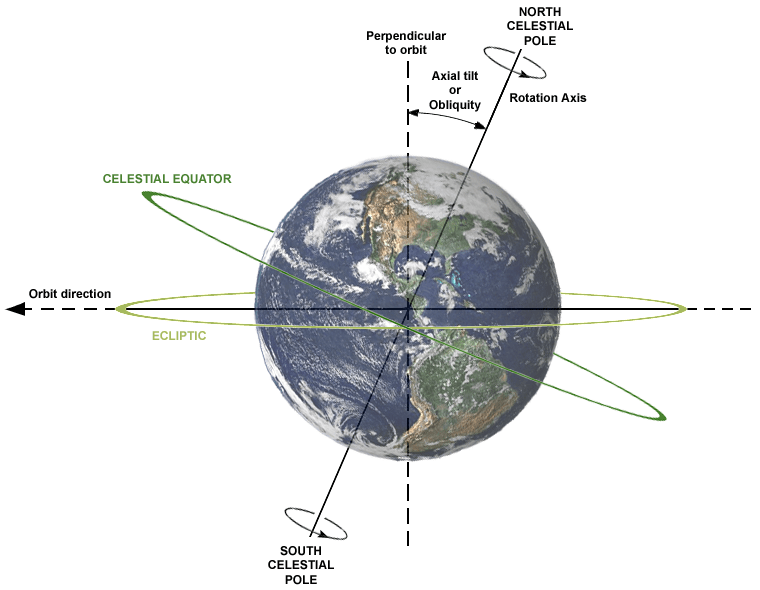
\includegraphics[width=100mm]{fig/earthOrbit}
    \caption{Detailschaltbild der Hardware}
\end{figure}
\begin{figure}[h]
    \centering
    % 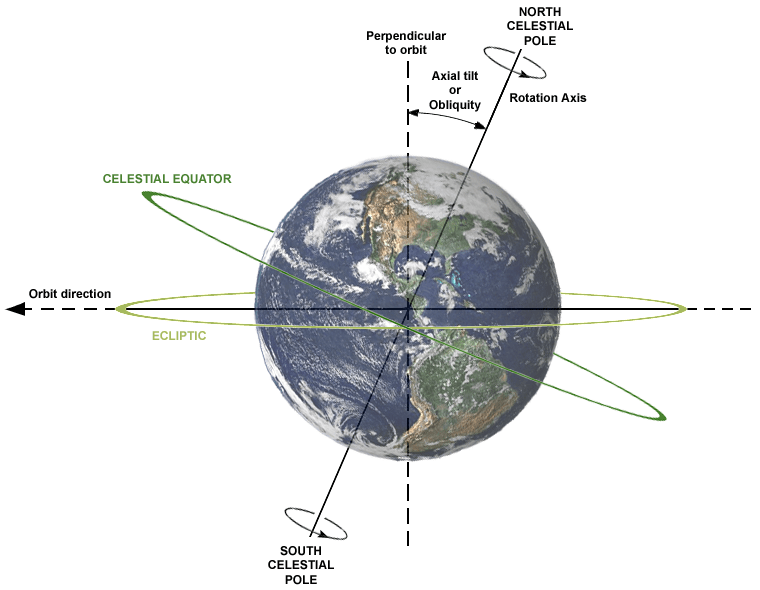
\includegraphics[width=100mm]{fig/earthOrbit}
    \caption{Beschreibung des Human Machine Interfaces}
\end{figure}
\clearpage

\subsection{Struktogramm der Software}
Hier wird beschrieben, wie die Software arbeiten soll!
Am besten ist die graphische Darstellung mittels Struktogramm oder Flussdiagramm.
Auch die Darstellung eines Zustandsdiagramms kann sinnvoll sein.
\begin{figure}[h]
    \centering
    % 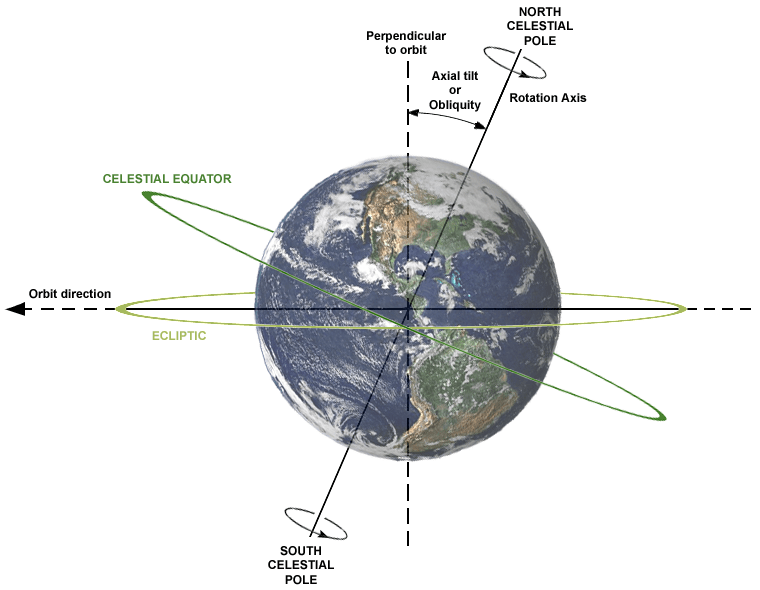
\includegraphics[width=100mm]{fig/earthOrbit}
    \caption{Struktogramm der Software}
\end{figure}
\begin{figure}[h]
    \centering
    % 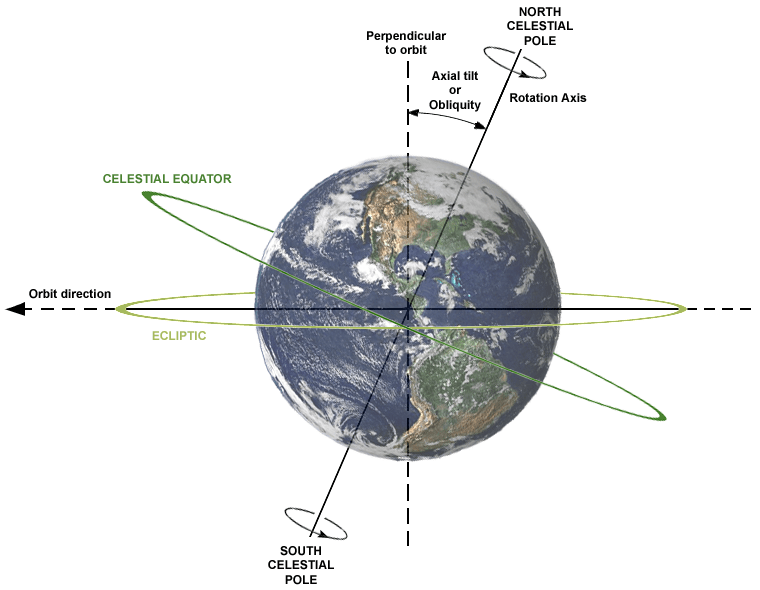
\includegraphics[width=100mm]{fig/earthOrbit}
    \caption{Zustandsdiagramm}
\end{figure}
\begin{figure}[h]
    \centering
    % 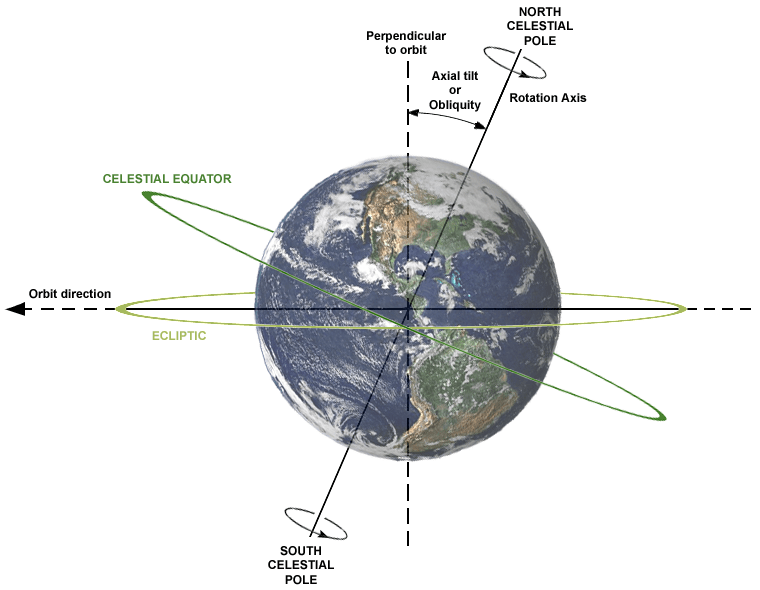
\includegraphics[width=100mm]{fig/earthOrbit}
    \caption{Beschreibung des Human Machine Interfaces}
\end{figure}
\clearpage

\section{Aufwände}
\subsection{Zeitliche Meilensteine in der Projektabwicklung}
Abschätzung der zeitlichen Durchführung anhand eines einfachen tabellarischen Projektablaufplanes.
Dabei soll für jeden Projektmitarbeiter eine Tabelle erstellt werden. \\
Die Planung muss zu Beginn nicht besonders detailreich sein, sie kann später noch verfeinert werden.
Außerdem kann hier zusätzlich eine Grafik von z.B. MS-Project eingefügt werden.

\subsubsection{Projektmitarbeiter 1}
\begin{tabularx}{\textwidth}{| l | X |}
    \hline
    \textbf{Datum} & \textbf{Meilenstein} \\
    \hline
     & \\
    \hline
\end{tabularx}

\subsubsection{Projektmitarbeiter 2}
\begin{tabularx}{\textwidth}{| l | X |}
    \hline
    \textbf{Datum} & \textbf{Meilenstein} \\
    \hline
     & \\
    \hline
\end{tabularx}

\subsection{Finanzielle Aufwendungen}
Auflistung der HW und SW Komponenten mit erster Abschätzung der Kosten. \\
\begin{tabularx}{\textwidth}{| p{0.06\textwidth} | p{0.4\textwidth} | p{0.3\textwidth} | X |}
    \hline
    \textbf{Pos.} & \textbf{Beschreibung} & \textbf{Bezugsquelle} & \textbf{Kosten}\\
    \hline
    1 & & & \\
    \hline
    2 & & & \\
    \hline
\end{tabularx}

\subsection{Sonstige Aufwendungen}
Sollte ein Projekt mit externen Partnern durchgeführt werden, so sind eventuell Reisekosten und zusätzlicher Kommunikationsaufwand hier zu beschreiben.

\clearpage
\listoffigures

\end{document}